Esta seção apresenta a metodologia de execução do presente trabalho.
A Seção \ref{subsec:classificacao} define o escopo e os objetivos deste trabalho, delineando as principais áreas de investigação.
Em seguida, a Seção \ref{subsec:metodologia} descreve as abordagens e técnicas utilizadas para planejar e conduzir o desenvolvimento da ferramenta proposta.
Por fim, a Seção \ref{subsec:solucao} detalha os passos do trabalho, incluindo a investigação da estrutura dos dados, a modelagem lógica e o desenvolvimento da ferramenta de integração de dados.

\section{Classificação da Pesquisa} \label{subsec:classificacao}

Para fundamentar a classificação metodológica da pesquisa, foram consultadas as obras de \citet{cervo:1983:metodologia}, que apresentam diferentes abordagens científicas, e de \citet{gerhardt:2009:metodos}, que tratam de métodos amplamente utilizados na pesquisa acadêmica.

Quanto à natureza, esta pesquisa é aplicada, pois busca resolver um problema prático relacionado à integração automatizada de dados financeiros públicos disponibilizados pela CVM, promovendo avanços na análise fundamentalista e no apoio à tomada de decisão.

Em relação aos objetivos, a investigação é exploratória e descritiva. A parte exploratória está ligada à compreensão da estrutura dos dados da CVM, enquanto o aspecto descritivo se manifesta na proposição e implementação de uma ferramenta que permita o uso prático dessas informações de forma organizada.

Os procedimentos técnicos combinam pesquisa bibliográfica e documental para levantamento e compreensão teórica dos dados públicos, juntamente com o desenvolvimento de uma solução tecnológica que automatiza sua coleta, integração e disponibilização.

A abordagem metodológica adotada é mista. Aspectos qualitativos estão presentes na análise estrutural e na modelagem dos dados, enquanto os elementos quantitativos se refletem no processamento automatizado e na organização das informações em larga escala.

No contexto da área de Computação, a pesquisa representa o desenvolvimento de uma solução tecnológica voltada à resolução de um problema específico, com potencial de aplicação prática no meio acadêmico e no ambiente de análise financeira \cite{wazlawick:2009:metodo}.


\section{Gerenciamento do Projeto} \label{subsec:metodologia}

O gerenciamento deste projeto foi conduzido com base em práticas ágeis de desenvolvimento de software, adotando a metodologia \textit{Scrum} como estrutura principal \cite{schwaber:2004:agile}. Como apoio visual, utilizou-se também o quadro de sinalização \textit{Kanban}, contribuindo para a organização e o acompanhamento do fluxo de trabalho \cite{anderson:2010:kanban}.

Ambas as abordagens foram aplicadas de forma adaptada às necessidades do projeto, considerando sua natureza acadêmica e o escopo restrito da equipe envolvida. O \textit{Scrum} foi utilizado de maneira personalizada, com ciclos iterativos de duas semanas, denominados \textit{sprints}, nos quais as tarefas foram definidas, priorizadas e acompanhadas ao longo do desenvolvimento \cite{sutherland:2014:scrum}.

O Kanban complementou esse processo, funcionando como ferramenta visual para monitoramento das atividades, identificação de gargalos e ajustes de fluxo, contribuindo para uma gestão mais eficiente \cite{hammarberg:2014:kanban}. Essa combinação flexível e adaptada de métodos ágeis mostrou-se eficaz para garantir a organização, a visibilidade do progresso e a entrega incremental da solução proposta.



\section{Solução proposta}  \label{subsec:solucao}

O ponto de partida do projeto consistiu em uma investigação detalhada da estrutura dos dados disponibilizados pela CVM. Essa etapa contemplou a análise dos formatos de arquivos, dos tipos de dados disponíveis e dos métodos de acesso às informações públicas fornecidas por essa instituição.

Embora os dados da B3 não tenham sido utilizados diretamente na construção da ferramenta, sua presença no contexto do mercado de capitais justificou a compreensão de sua estrutura e funcionamento. Dessa forma, foram consultados documentos como o relatório anual da CVM \cite{cvm:2023:relatorioanual} e referências sobre a estrutura de dados da B3 \cite{b3:2023:estruturadados}, a fim de mapear desafios e possibilidades associados à integração de dados financeiros.

A Figura \ref{fig:fluxograma} ilustra o fluxo geral do projeto. A fase inicial compreendeu a coleta e documentação dos dados da CVM, seguida pela modelagem lógica que estruturou um banco de dados unificado, preparado para integração e análise posterior.

\begin{figure}[!htb] \centering
	\caption{Fluxograma do projeto} \label{fig:fluxograma}
	\begin{varwidth}{\linewidth}
		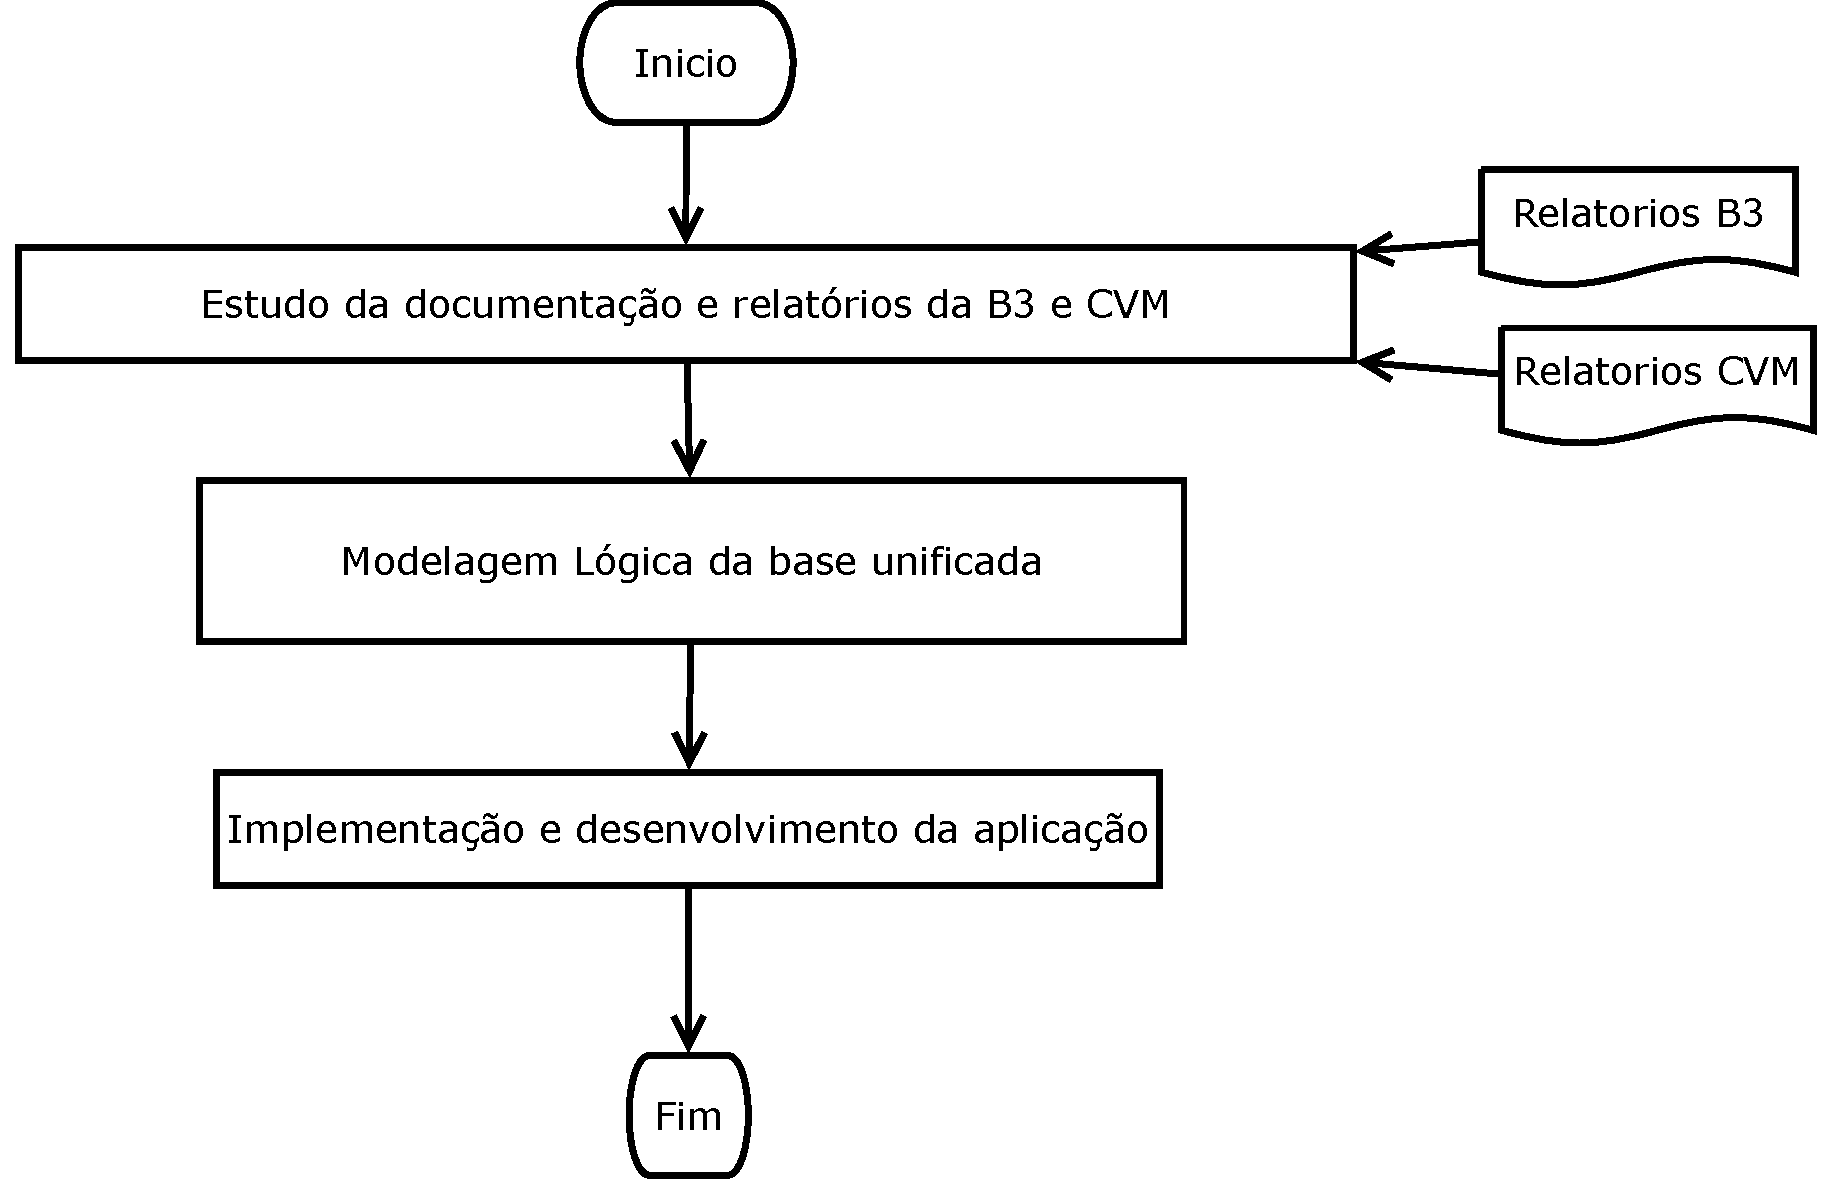
\includegraphics[width=0.6\textwidth]{figuras/fluxograma - v3.pdf}
		\legend{Elaborado pelo autor, 2024.}
	\end{varwidth}
\end{figure}

Com base na análise inicial, foi realizada a modelagem lógica da base de dados, com foco na criação de um esquema unificado que contemplasse as diferentes estruturas contábeis e financeiras presentes nos arquivos da CVM. Para essa etapa, foram consideradas boas práticas descritas na literatura sobre modelagem de dados financeiros \cite{domingues:2020:modelagem} e integração de grandes volumes de dados \cite{perlin:2021:analise}.

A etapa seguinte consistiu no desenvolvimento da aplicação de software responsável por automatizar o processo de coleta, tratamento e inserção dos dados na base unificada. Essa ferramenta foi desenvolvida com tecnologias modernas de extração e processamento de dados, garantindo flexibilidade e desempenho.

A aplicação foi capaz de realizar o download dos arquivos disponibilizados pela CVM, aplicar os tratamentos necessários para padronização e limpeza dos dados, e armazená-los de forma estruturada. Esse processo assegurou a integridade das informações e facilitou seu uso em análises fundamentalistas, estudos acadêmicos e outras aplicações. A proposta esteve alinhada com práticas consolidadas no desenvolvimento de soluções para automação e análise de dados \cite{prikladnicki:2014:desenvolvimentosoftware} \cite{nhimi:2016:desenvolvimentosoftware}.


\section{Materiais e Tecnologias} \label{subsec:material}

Esta seção apresenta os materiais e tecnologias que serão empregados durante o desenvolvimento do trabalho.  
O projeto será desenvolvido em um computador desktop cujas especificações são apresentadas no Quadro \ref{tab:specs-tcc}.  


\begin{board}[!htb]  \centering
	\caption{Especificações do computador utilizado no TCC}
	\label{tab:specs-tcc}
	\begin{varwidth}{\linewidth}
		\begin{tabular}{|p{4cm}|p{11cm}|} \hline
			\textbf{Componente} & \textbf{Especificação} \\ \hline
			Processador & AMD Ryzen 5 5600G, 6-Core, 12-Threads, 3.6GHz (4.6GHz Turbo), Cache 19MB, AM4 \\ \hline  
			Memória RAM & 2x Kingston Fury Beast, 16GB, 3200MHz, DDR4, CL16 \\ \hline  
			Armazenamento & SSD TGT Seal ST, 240GB, Sata III, Leitura 500 MB/s, Gravação 450 MB/s \\  
			& HD WD Blue, 1TB, 3.5, 5400 RPM, Sata III, Cache 64MB \\ \hline  
			Sistema Operacional & Windows 11 Pro \\ \hline
		\end{tabular}
		\legend{Elaborado pelo autor, 2024.}
	\end{varwidth}
\end{board}

Durante a modelagem do banco de dados, utilizou-se o MySQL Workbench\footnote{\url{https://www.mysql.com/products/workbench/}}, versão 8.0. Essa ferramenta permitiu a criação visual do esquema lógico, facilitando o planejamento e a organização das entidades e relacionamentos.

Contudo, para o desenvolvimento da aplicação, optou-se pelo uso do SQLite\footnote{\url{https://www.sqlite.org/}}, versão 3.49.1, como solução de banco de dados local. O SQLite foi adotado como banco de dados padrão do sistema, por oferecer maior praticidade na integração com o código desenvolvido. Sua leveza, portabilidade e independência de um servidor o tornam especialmente adequado para o uso do código por estudantes e profissionais da área financeira.

A linguagem de programação utilizada foi o Python, na versão 3.12.9\footnote{\url{https://www.python.org/downloads/release/python-3129/}}, pela sua versatilidade, ampla comunidade e bibliotecas especializadas.

As bibliotecas utilizadas no projeto foram:

\begin{itemize}
	\item Pandas, versão 2.2.1\footnote{\url{https://pandas.pydata.org/}}
	\item Numpy, versão 1.26.4\footnote{\url{https://numpy.org/}}
	\item Beautifulsoup4, versão 4.12.2\footnote{\url{https://www.crummy.com/software/BeautifulSoup/}}
	\item Lxml, versão 5.1.0\footnote{\url{https://lxml.de/}}
	\item Requests, versão 2.31.0\footnote{\url{https://requests.readthedocs.io/en/latest/}}
	\item SQLAlchemy, versão 2.0.27\footnote{\url{https://www.sqlalchemy.org/}}
	\item Mysql-Connector-Python, versão 8.3.0\footnote{\url{https://dev.mysql.com/downloads/connector/python/}}
\end{itemize}

A biblioteca \textit{pandas} foi empregada para manipulação e análise de dados tabulares. Sua estrutura baseada em \textit{DataFrames} proporcionou uma forma eficiente de organizar, filtrar e agrupar informações financeiras.

A biblioteca \textit{numpy} foi utilizada em conjunto com o pandas para operações numéricas vetoriais e matriciais, fundamentais na realização de cálculos e no tratamento de grandes volumes de dados.

Para extração de informações de páginas web, foi utilizada a biblioteca \textit{beautifulsoup4}, que permitiu navegar pela estrutura HTML de documentos e extrair dados de forma precisa. A ela foi integrada a biblioteca \textit{lxml}, que serviu como parser rápido e eficiente de HTML e XML.

A coleta dos dados disponibilizados pela CVM foi realizada por meio da biblioteca \textit{requests}, que viabilizou a comunicação com serviços HTTP e o download automatizado das informações necessárias.

A interface com o banco de dados foi desenvolvida com o auxílio do \textit{SQLAlchemy}, que forneceu abstração e controle sobre as operações de inserção, consulta e atualização dos dados no SQLite, utilizando o paradigma de mapeamento objeto-relacional.

%Texto antigo
%Durante os testes iniciais com a estrutura modelada no MySQL, foi utilizada a biblioteca \textit{mysql-connector-python}, o conector oficial do MySQL para Python. Essa ferramenta garantiu a compatibilidade entre a modelagem relacional inicial e os scripts desenvolvidos, possibilitando a validação funcional da estrutura antes da migração definitiva para o SQLite.
%
%A escolha pelo banco de dados SQLite justifica-se por sua leveza, portabilidade e facilidade de integração com sistemas locais, características adequadas a estudos exploratórios e reprodutíveis.

%Texto novo
Durante a fase inicial de testes com a estrutura relacional modelada em MySQL, utilizou-se a biblioteca \textit{mysql-connector-python}, conector oficial disponibilizado para integração entre aplicações Python e bancos de dados MySQL. Essa ferramenta assegurou plena compatibilidade entre o modelo relacional e os \textit{scripts} desenvolvidos, permitindo validar o funcionamento da estrutura proposta em um ambiente robusto e amplamente utilizado no contexto de bancos relacionais.

Após essa etapa de validação, optou-se pela migração definitiva para o banco de dados SQLite. A escolha por essa tecnologia deve-se à sua leveza, portabilidade e facilidade de integração com sistemas locais, características particularmente vantajosas para estudos exploratórios, reproduzíveis e com foco acadêmico ou experimental, como é o caso deste trabalho.